\chapter{CAD-Konstruktion}

\section{Setup und Einarbeitung (Becker, Specht)}

Zu Beginn des Projekts wurde in Abstimmung mit Fabian Becker sowie im Austausch mit Andreas Wittmann (Studienkollege) entschieden, FreeCAD als CAD-Software zu verwenden. Der Grund hierfür war die einfache Kollaboration innerhalb der Projektgruppe sowie der unkomplizierte Erfahrungsaustausch mit der Arbeitsgruppe um A. Wittmann. Andere Softwarelösungen wie OnShape wurden diskutiert, aufgrund der Komplexität und der damit verbundenen Einarbeitungszeit im Hinblick auf die Projektlaufzeit jedoch verworfen. FreeCAD ist zudem eine Open-Source-Software, die neben Fedora auch auf Debian-Systemen lauffähig ist. So konnte die Software problemlos auf den Arbeitsrechnern der Teammitglieder installiert werden.

Grundsätzlich stützt sich die Konstruktion auf vorhandene STL-Vorlagen. Ein Beispielprojekt aus dem Internet diente als Grundlage für die Arbeit.

\section{Geschützarm Version 1 (Specht) \label{sec:cad_gunarm_v1}}

Bevor mit der Konstruktion begonne wurde, wurde im Team besprochen, welche Komponenten nötig sind, um die Position des Flugobjekts eindeutig zu bestimmen. Die Wahl fiel auf folgende Komponenten, die aus vorherigen Studienprojekten übernommen werden konnten:

\begin{itemize}
    \item GY-521 MPU-6050 3-Achsen-Gyroskop und Beschleunigungssensor
    \item SRF02 Ultraschall Entfernungssensor
    \item Raspberry Pi 5 Kamera Modul
    \item 2x 28BYJ-48 Schrittmotor
\end{itemize}

Ziel des ersten Entwurfs war es, diese kompakt auf dem Arm zu integrieren. Die angedachten Schrittmotoren wichen jedoch von der Vorlage aus dem Beispielprojekt ab, weshalb der Geschützarm von Grund auf neu konstruiert werden musste.

Alle Module sollten zentral über der Abschusseinrichtung platziert werden, um eine korrekte Berechnung der Flugbahn zu ermöglichen. Der Ultraschall-Sensor sollte dabei hochkant nach vorne gerichtet sein, um die Entfernung zum Ziel zu messen. Die Kamera sollte schräg nach oben gerichtet sein, um den Himmel zu überwachen. Der Beschleunigungssensor sollte liegend auf dem Arm montiert werden, um die Beschleunigung des Arms zu messen. Die Schrittmotoren mussten in einem geeigneten Abstand zueinander montiert werden, sodass die Flywheel-Konstruktion des Arms funktioniert. Letzteres konnte durch das Vermessen der Vorlage aus dem Beispielprojekt realisiert werden. Für die restlichen Anforderungen waren die korrekten Maße nötig. Für die Montage der Kamera konnte eine bereits 3D-gedruckte Halterung aus einer anderen Gruppe benutzt werden. Die Haltevorrichtung für den Beschleunigungssensor wurde aus einer STL-Vorlage übernommen und angepasst. Auch für die Schrittmotoren konnte auf ein Modell aus dem Internet zurückgegriffen werden, weshalb es nicht nötig war, die komplexe Geometrie eigenständig zu vermessen. Einzig die Maße für den Ultraschall-Sensor wurden recherchiert und durch Nachmessen validiert.

\begin{figure}[h]
    \centering

    \begin{subfigure}[b]{0.45\textwidth}
        \centering
        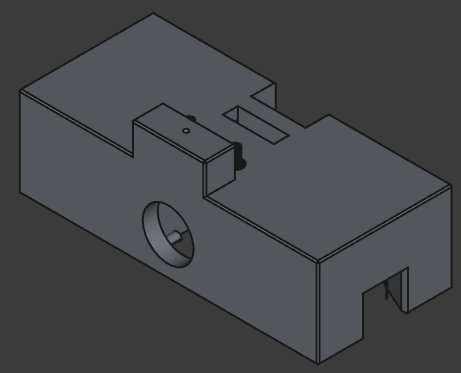
\includegraphics[width=\textwidth]{images/cad_gunarm_v1_front.jpg}
        \caption{Geschützarm Version 1 - Frontansicht}
    \end{subfigure}
    \hfill
    \begin{subfigure}[b]{0.45\textwidth}
        \centering
        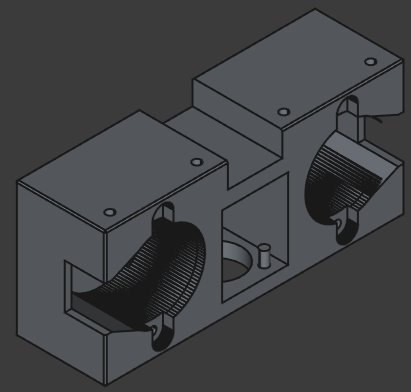
\includegraphics[width=\textwidth]{images/cad_gunarm_v1_back.jpg}
        \caption{Geschützarm Version 1 - Rückansicht}
    \end{subfigure}

    \caption{Geschützarm Version 1}
    \label{fig:gunarm_v1}
\end{figure}

Neben den eigentlichen Maßen der Komponenten war das Kabelmanagement ein wichtiges Thema. Alle Kabel sollten nach hinten am Magazin entlang geführt werden, um eine saubere Optik zu gewährleisten. Für Beschleunigungssensor und Kamera stellte dies kein Problem dar, da diese ganz oben angebracht sein sollten. Der Ultraschall-Sensor und die Schrittmotoren hingegen waren in das neukonstruierte Gehäuse integriert, sodass Aussparungen, wie in Abbildung~\ref{fig:gunarm_v1} zu sehen, angebracht werden mussten, um die Kabel aus dem Gehäuse herauszuführen.

Außerdem musste sichergestellt werden, dass der Geschützarm an das Magazin montiert werden kann. Hierzu wurden vom Kollegen Fabian Becker Montagepunkte am Magazin konstruiert, die mit dem Geschützarm verschraubt werden können.

\section{Geschützarm Version 2 (Specht)}

Im Laufe des Projektes wurde in Abstimmung mit Fabian Becker klar, dass die Schrittmotoren aufgrund zu geringer Leistung nicht für die Flywheel-Konstruktion geeignet sind. Daraufhin wurde sich für die originalen Motoren aus dem Beispielprojekt entschieden. Das hatte zur Folge, dass der Geschützarm neu konstruiert werden musste, da die Maße der neuen Motoren von den Alten abwichen. Aus diesem Grund wurde der Geschützarm der Vorlage als Basis genommen und die Grundidee der Version 1 beibehalten.

\begin{figure}[h]
    \centering

    \begin{subfigure}[b]{0.45\textwidth}
        \centering
        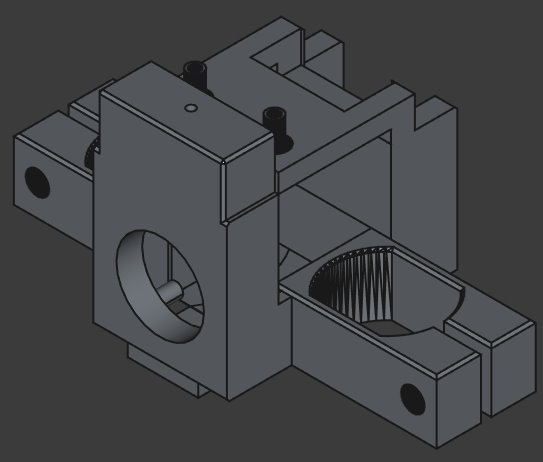
\includegraphics[width=\textwidth]{images/cad_gunarm_v2_front.jpg}
        \caption{Geschützarm Version 2 - Frontansicht}
    \end{subfigure}
    \hfill
    \begin{subfigure}[b]{0.45\textwidth}
        \centering
        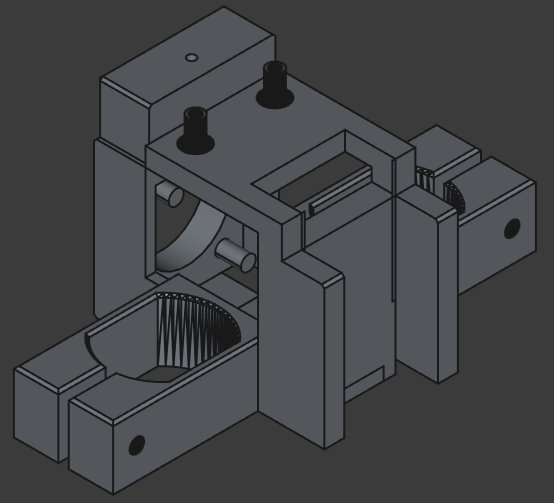
\includegraphics[width=\textwidth]{images/cad_gunarm_v2_back.jpg}
        \caption{Geschützarm Version 2 - Rückansicht}
    \end{subfigure}

    \caption{Geschützarm Version 2}
    \label{fig:gunarm_v2}
\end{figure}

Im Gegensatz zur Version 1 wird der Ultraschallsensor nun seitlich eingeführt anstatt von unten, siehe~\ref{fig:gunarm_v2}. Problematisch waren dabei die beschränkten Platzverhältnisse, da die Schrittmotoren näher am Kanonenrohr angebracht wurden als im vorherigen Entwurf. Außerdem wurden die zuvor angedachten Montagepunkte am Magazin wieder entfernt. Die Zusammenführung des Geschützarms mit dem Magazin erfolgte deshalb mittels Modellbaukleber.

\section{Montagehalterung Motortreiber (Specht)}

Für die ersten Funktionstests wurden die Pololu-Motoren provisorisch auf Kork-Schnipseln montiert. Dieses Vorgehen ermöglichte eine zügige Inbetriebnahme, jedoch erwies es sich hinsichtlich Stabilität und Sicherheit als unzureichend. Im Rahmen der Tests kam es zum Abrutschen eines Motors von der Korkunterlage, was zu einer kurzfristigen Wärmeentwicklung und Geruchsbildung führte. Glücklicherweise wurde eine Beschädigung der Hardware vermieden.

\begin{figure}[h]
    \centering

    \begin{subfigure}[b]{0.25\textwidth}
        \centering
        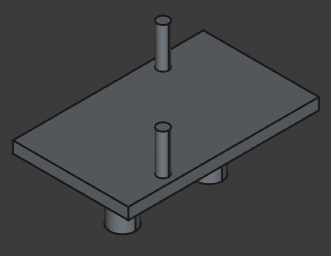
\includegraphics[width=\textwidth]{images/cad_polulu_front.png}
        \caption{Polulu - Draufsicht}
    \end{subfigure}
    \hspace{0.05\textwidth} % Adjust this value as needed
    \begin{subfigure}[b]{0.25\textwidth}
        \centering
        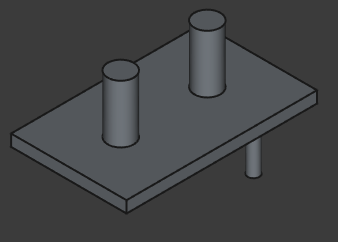
\includegraphics[width=\textwidth]{images/cad_polulu_back.png}
        \caption{Polulu - Bodensicht}
    \end{subfigure}

    \caption{Montagehalterung für Pololu-Motortreiber}
    \label{fig:pololu_mounting}
\end{figure}

Für die finale Abnahme wurde daher ein dauerhaftes und sicheres Montagesystem umgesetzt, das ein sauberes und zuverlässiges Setup gewährleistet. Wie in Abbildung~\ref{fig:pololu_mounting} zu sehen, kann die Halterung direkt auf der Montageplatte des Fahrzeugs geklippt werden.